\documentclass[12pt,twoside]{rif}

\pagestyle{myheadings}
\usepackage[
left=2.54cm,
right=2.54cm,
top=2.54cm,
bottom=2.54cm]
{geometry}
\usepackage{hyperref}
\usepackage{natbib}
\usepackage{subfigure}
\hypersetup{
	urlcolor=blue, 
	colorlinks=true, 
	citecolor=blue
}

\usepackage{lipsum}

\title{\textbf{Dilatación del tiempo gravitacional}}

\author[1]{{\small Carlos Andrés García Suarez}} 
\author[1]{{\small David Brandon Zevallos Garay}}
\author[1]{{\small Luis Fernando Ubillus Benites}}
%\author[3]{Autor3}
\affil[1]{{ \small Facultad de Ciencias Naturales y Matemática, Universidad
		Nacional Federico Villarreal. El Agustino 15003. Lima-Perú.}}
%\affil[2,3]{Afiliacion2}
%\date{\normalsize Recibido: xxxx Aceptado: xxxx Publicado: xxxx\\
%Todos los derechos reservados-SEF \copyright{} 2012}
\date{}

\begin{document}
	\maketitle
	
	\begin{res}
		\begin{center}
			\textbf{Resumen} \\
		\end{center}
		\lipsum[2]
		
		\par
		\smallskip
		\clav{sdjssasdfsdf, asdfsdf, asdfsdafsd}
	\end{res}
	\begin{center}
		\title{\textbf{Time gravitational dilation}}
	\end{center}
	
	\begin{abst}
		\begin{center}
			\textbf{Abstract} \\
		\end{center}
		\lipsum[2]
		
		\par 
		\smallskip
		\key{sdjssasdfsdf, asdfsdf, asdfsdafsd}
	\end{abst}

	
	
	\newpage
	
	\tableofcontents
	
	\section{ Introducción} 
	La teoria de la relativida especial (RE) es una de las teorias 'anti intuitivas' del siglo XIX junto con la Mecanica
Cuantica, la RE nos da una comprension del universo a medidas macroscopicas para sistemas inerciales, Esta nos da un nuevo
concepto del Espacio y el tiempo Newtoniano, juntado como un solo ente llamado Espacio-Tiempo. (14)
Esta tenia como limites los marcos inerciales (no acelerado con respecto a otro) en 1907 se dio cuenta de la
incompatibilidad con la gravedad Newtoniana, impresionado por la igualdad inercial y gravitatoria debido al experimento 
como el de Lorand Eotvos (2) y mejorado en 1964 por Robert Dicke (3) se sabe que eran equivalentes ambas definiciones de masa.
En 1907 mas tarde se dio cuenta que: \\

 'un observador en caida libre no siente su propio peso y por lo tanto podria pensar que estuviera en una region del espacio donde no hubiera campo gravitarorio' (4) (copia literal)\\

Con este principio pudo generalizar el concepto de observador inercial y obtener las ecuaciones de campo de Einstein que dan
una descripcion de como el espacio-tiempo le dice al "ente" como moverse y como el "ente" deforma el espacio-tiempo(5)
Se hicieron diversos experimentos para comprobar lo que dice la Relatividad General en los limites Newtonianos, uno de ellos 
es el experiento de  Pound y Rebka (6) y en 1964 el experimento de Pound-Snider (7) del corrimiento al rojo de fotones que
escapan de un potencial gravitatorio.
En la epoca actual una aplicacion conocida es la del GPS que tiene que realizar correciones relativista para conseguir la 
sincronizacion (8) o el corrimiento al rojo de las enanas blancas, estudio llevado a cabo en una tesis con datos recopilados de 
Distintas Bases de datos de enanas blancas (9)
	\section{Marco Teórico}
	\subsection{Teoria de la Relatividad Especial}
	Este es el enfoque moderno que le dio Albert Einsten a la fisica, donde se "olvida" el concepto de tiempo y distancia Absoluto de la Teoria de Newton.
	Esta teoria se basa en dos postulados simplemente:
	Las leyes de la Fisica son validas para todos los sistemas "inerciales"
	 La velocidad de la luz en el vacio es igual para todos los observadores 
	Hay que tener cuidado con la palabra inercial que es su campo de aplicacion.
	\subsection{Principio de equivalencia}
	Un punto clave en este trabajo es el principio de equivalencia, que nos dice que un observador en caida libre en un campo gravitatorio es equivalente a un observador en el espacio fuera de toda influencia gravitatoria. Todo esto de forma local hasta que este sienta las consecuencias de la curvatura. Pero tambien nos dicen que un observador acelerado con aceleracion a en el espacio sin influencia de gravedad,es equivalente a un observador inercial en tierra con una gravedad igual a -a. Todo esto de forma local, hasta que el observador en el espacio se de cuenta que no sigue una geodesica.
	\subsection{Principio de Covariancia}
	"Este principio nos indica que el lenguaje tensorial permite escribir las leyes de la Fisica de manera que son validas para todos los observadores." (Expo2,pag 151)
	\subsection{Sistema Inecial}
	Dado que para Newton un Sistema inercial es aquel que tiene una velocidad relativa a otro en reposo, para este estaba bien definido este concepto, pero gracias al principio de equivalencia se observa que un observador acelerado tambien se puede considerar a si mismo como inercial por lo menos de forma local...
	\subsection{Relatividad General y Solucion de Scharwschild}
	Deducir la dilatacion para un universo vacio,estatico.
	
	\section{Aplicaciones}
	
	\subsection{GPS}
	Una de las aplicaciones mas conocidas es en GPS, donde este necesita unas correcciones relativistas, tanto especial como general, para conseguir la sincronizacion de los relojes en cada punto de la tierra y los satelites
	(Referir al articulo GPS2)
		\begin{center}
		\begin{figure}
		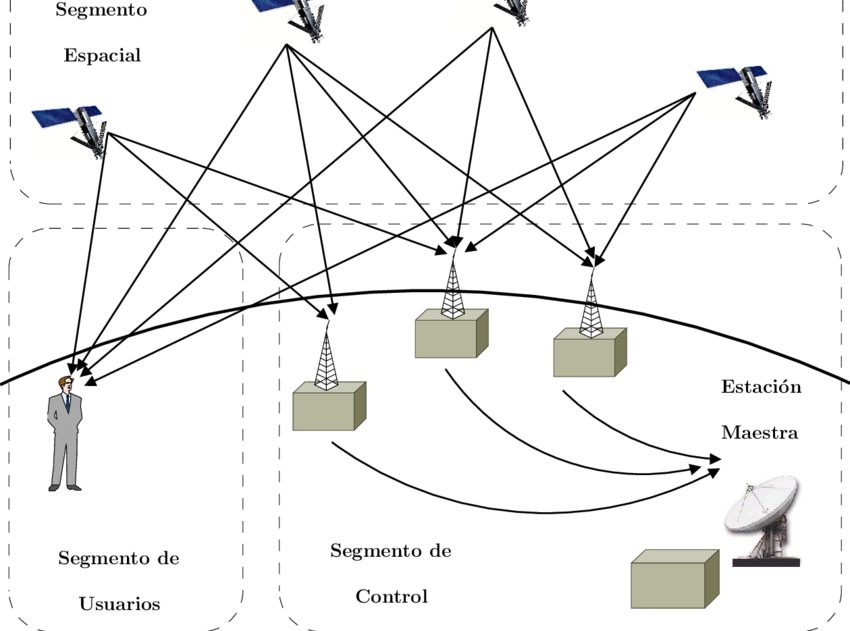
\includegraphics[width=0.8\textwidth]{img/GPS.png}
		\end{figure}
		\end{center}
	\subsection{Astrobiologia}
	Nosotros no observaremos el mismo comportamiento aqui que en  el espacio(visto desde Tierra)
	\section{Conclusiones}

	\nocite{*}
	\bibliographystyle{apa}
	\bibliography{biblio}
	

\end{document}